% 4:05 - 5:05
% 60 minutes

\begin{solutionbox}[Q1-1]

    \begin{center}
        \centering
        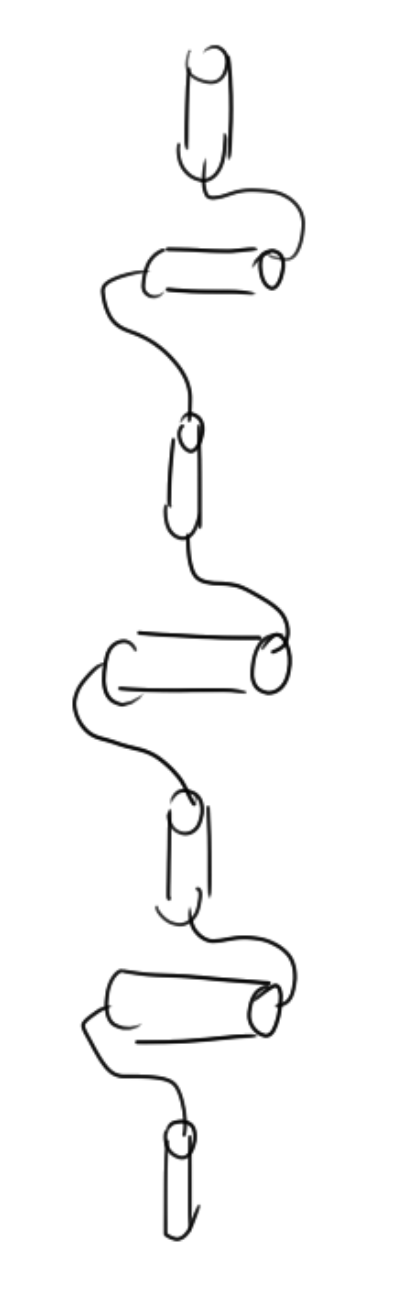
\includegraphics[height=120mm]{imgs/y2023-v1-q1-1.png}
    \end{center}

    There is a spherical wrist so when axis 5 and axis 7 lines up, there is a singularity.

    Alternatively, when the center of the spherical joint lines up with axis 1, there is a singularity. (alternative and equivalent is when axis 1, 5, and 7 coincide at same point)
\end{solutionbox}

\begin{solutionbox}[Q1-2-i]
    \begin{align*}
        {\,^0f}=
        \begin{bmatrix}
            0  & -c & b  \\
            c  & 0  & -a \\
            -b & a  & 0
        \end{bmatrix} \\
        \begin{bmatrix}
            0  & 4 & 3  \\
            -4 & 0 & -2 \\
            -3 & 2 & 0
        \end{bmatrix}
    \end{align*}
\end{solutionbox}

\begin{solutionbox}[Q1-2-ii]
    \begin{align*}
        C_1       & = C_0 {\,^0C_1} \\
        {\,^0C_1} & =
        \begin{bmatrix}
            1 & 0                  & 0                   \\
            0 & \frac{1}{\sqrt{2}} & -\frac{1}{\sqrt{2}} \\
            0 & \frac{1}{\sqrt{2}} & \frac{1}{\sqrt{2}}  \\
        \end{bmatrix}
    \end{align*}

    \begin{align*}
        {\,^1f}={\,^0C_1}^{T}{\,^0f}{\,^0C_1}
    \end{align*}

\end{solutionbox}

\begin{solutionbox}[Q1-2-iii]

    \begin{align*}
        \sqrt{1+4+9} = \sqrt{14}
    \end{align*}

    \begin{align*}
        e^{\pi/6\cdot \frac{1}{\sqrt{14}} \cdot \left(\begin{bmatrix}1\\-2\\3\end{bmatrix}\right)\times}
    \end{align*}
\end{solutionbox}

\begin{solutionbox}[Q1-3]
    \begin{align*}
        {\,^0w_{3,0}} = \dot{\theta_1} k + e^{\theta_1 k\times} \dot{\theta_2} j + e^{\theta_1 k\times} e^{\theta_2 j\times} \dot{\theta_3} i \\
    \end{align*}
\end{solutionbox}


\begin{solutionbox}[Q1-4]
    First generate the percentage of the way there should the robot be at any given time using a quintic polynomial. Then, at lerp between the positions and slerp between the orientation to find the target position and orientation at that "percent of the way there". Then use the target position and orientation as input to inverse kinematics.

    Quintic polynomial is used such that acceleration doesn't change rapidly aka there is no infinite jerk in the planned trajectory.
\end{solutionbox}

\begin{solutionbox}[Q1-5]
    \begin{align*}
        T & = \frac{1}{2} m \left(l\dot{\theta}\right)^2                    \\
        V & = mgl(-\cos\theta)                                              \\
        L & = T-V                                                           \\
        L & = \frac{1}{2} m \left(l\dot{\theta}\right)^2 - mgl(-\cos\theta) \\
        L & = \frac{1}{2} m \left(l\dot{\theta}\right)^2  +mgl\cos\theta    \\
    \end{align*}

    \begin{align*}
        \frac{d}{dt} \left( \frac{\partial L}{\partial \dot{\theta}} \right) - \frac{\partial L}{\partial \theta} & = \tau \\
        \frac{d}{dt} \left( ml^2\dot{\theta} \right) - (-mgl\sin\theta)                                           & = \tau \\
        ml^2\ddot{\theta} + mgl\sin\theta                                                                         & = \tau \\
    \end{align*}
\end{solutionbox}

\begin{solutionbox}[Q1-6]
    \begin{align*}
        \theta        & = \pi/2 (1-\cos\left(\pi/T \cdot t\right))    \\
        \dot{\theta}  & = \pi^2/(2T) \sin\left(\pi/T \cdot t\right)   \\
        \ddot{\theta} & = \pi^3/(2T^2) \cos\left(\pi/T \cdot t\right) \\
    \end{align*}
    \begin{align*}
        \tau & = ml^2\ddot{\theta} + mgl\sin\theta                                                                                \\
        \tau & = ml^2 \pi^3/(2T^2) \cos\left(\pi/T \cdot t\right) + mgl\sin\left(\pi/2 (1-\cos\left(\pi/T \cdot t\right)) \right) \\
    \end{align*}
\end{solutionbox}

\begin{solutionbox}[Q1-7]
    \begin{align*}
        G(q) = \begin{bmatrix}
                   m_2gd_2\sin(\theta_1) \\
                   -m_2g\cos(\theta_1)   \\
               \end{bmatrix}
    \end{align*}

    \begin{align*}
        D(q) = \begin{bmatrix}
                   m_2d_2^2 & 0   \\
                   0        & m_2 \\
               \end{bmatrix}
    \end{align*}

    \begin{align*}
        T & = \frac{1}{2}v^{T}D(q)v                                                \\
          & =
        \frac{1}{2}\begin{bmatrix}
                       \dot{\theta_1} & \dot{d_2} \\
                   \end{bmatrix}
        \begin{bmatrix}
            m_2d_2^2 & 0   \\
            0        & m_2 \\
        \end{bmatrix}
        \begin{bmatrix}
            \dot{\theta_1} \\
            \dot{d_2}      \\
        \end{bmatrix}                                                             \\
          & =
        \frac{1}{2}\begin{bmatrix}
                       \dot{\theta_1} & \dot{d_2} \\
                   \end{bmatrix}
        \begin{bmatrix}
            m_2d_2^2 \dot{\theta_1} \\
            m_2\dot{d_2}            \\
        \end{bmatrix}                                                    \\
          & = \frac{1}{2} m_2 d_2^2 \dot{\theta_1}^2 + \frac{1}{2} m_2 \dot{d_2}^2
    \end{align*}

\end{solutionbox}

\begin{solutionbox}[Q1-8]
    PD plus gravity is in joint space.

    Given desired $q_r$ and desired $\dot{q_r}$. $e_{q} = q_r-q$. $e_{qd} = \dot{q_r}-\dot{q}$. Get gravity term from the term on top, call it $u_g$ (this calculated from measured q). $u=kp\cdot e_q + kv\cdot e_{qd} + u_g$

    PD plus feedforward is the following.


    Given desired $q_r$ and desired $\dot{q_r}$. $e_{q} = q_r-q$. $e_{qd} = \dot{q_r}-\dot{q}$. Get all the torques from the equations of motion and call that $u_{ff}$. (this uses desire $q$, desired $\dot{q}$, and desired $\ddot{q}$) $u=kp\cdot e_q + kv\cdot e_{qd} + u_{ff}$
\end{solutionbox}

\begin{solutionbox}[Q1-9]
    BFS, not gonna to elaborate.
\end{solutionbox}

\begin{solutionbox}[Q1-10]
    The color match experiment is to figure out how human retina responds to the three primaries colors RGB. Given example in class for color processing is to remove the effect of lighting and shadow when trying to identify the road.

    \boxbar
    Camera calibration is necessary to get both the intrinsic and extrinsic parameters which are (focal length, principle point, field of view, and camera distortion) and (rotation and translation vectors WRT world coordinates). Using the camera calibration tool box, about 20 is needed.

    \boxbar
    Template matching is used to find some small image in a large image. It can be used to play some 2d video games (like Super Mario bros) to detect the appearance of specific enemies since the sprites are easily known.

    \boxbar
    Morphological operation of opening is erosion (expanding black regions) followed by dilations (expanding white regions). The combined effect is that the related size of the black and white regions berely changes, but the small white particles are removed from the image. Closing is the exact opposite as it dilates first than erode which removes small black points.

    \boxbar
    (a), (c) are true. Someone may use (b) to decrease salt and pepper noise followed by a rounding operation. Though morphological operation is more often used. Corners use a different algorithm
\end{solutionbox}